\documentclass{article}
\usepackage{graphicx}
\usepackage[letterpaper, margin=1.25in]{geometry}

\setlength\parindent{0pt}

\begin{document}
\subsection*{Two Cuts}

\centerline{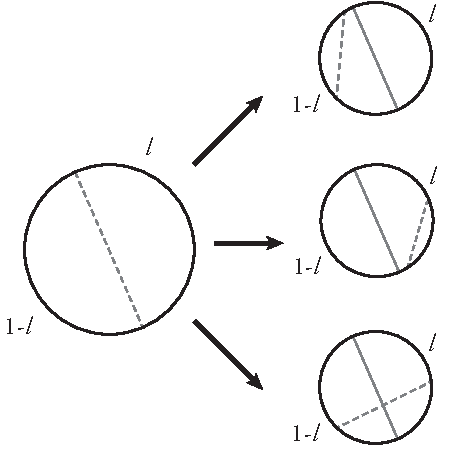
\includegraphics[scale = 0.75]{Slice-2Cut.pdf}}

After the pizza is cut once, we can easily find the probability that the second cut will lead to three pieces vs. four pieces and use this to calculate the expected value of pieces.
$$ \mathrm{Probability~of~3~Pieces:~} p_{3(2)} = \int_0^1 l^2 + (1 - l)^2 dl = \left. \frac{2l^3}{3} - l^2 + l \right\vert_0^1 = \frac{2}{3}$$
$$ \mathrm{Probability~of~4~Pieces:~} p_{4(2)} = \int_0^1 2l(1 - l) dl = \left. -\frac{2l^3}{3} + l^2 \right\vert_0^1 = \frac{1}{3}$$
$$ \mathrm{Expected~value~of~pieces~=~} 3\left(\frac{2}{3}\right) + 4\left(\frac{1}{3}\right) = 3\frac{1}{3}$$

\subsection*{Three Cuts}

\centerline{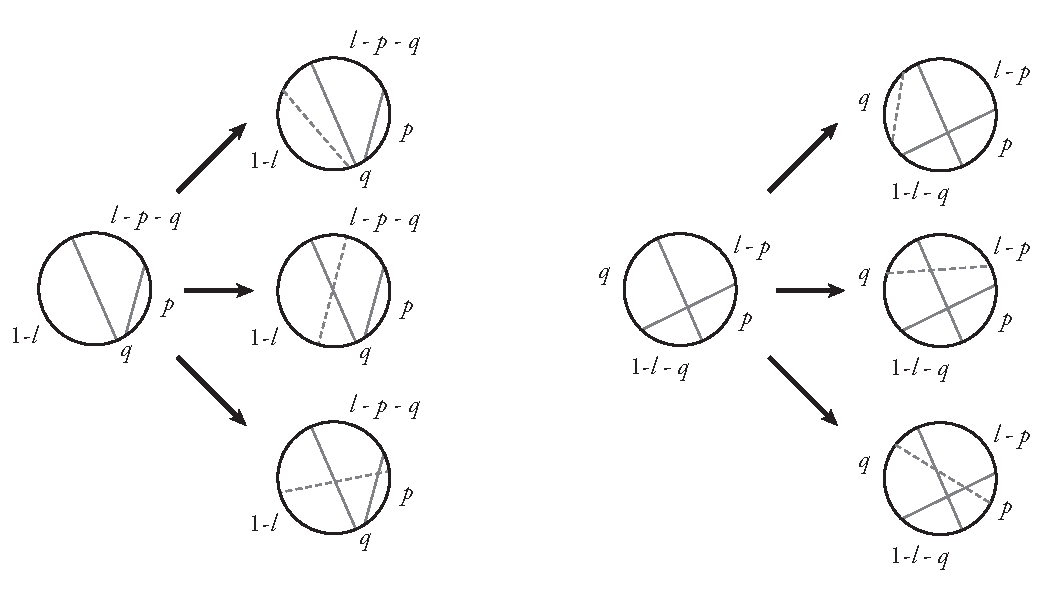
\includegraphics[scale = 0.75]{Slice-3Cut.pdf}}

\pagebreak

Given that we have already solved the case of two cuts, we simply need to deal with all the scenarios that branch out from there. Thus, we can calculate the relative likelihood for 4, 5, and 6 pieces after three cuts, when after two cuts, there are only three pieces:

$$4: \alpha = \int_0^1 \int_0^l \int_0^{l - q} p^2 + q^2 + (l - p - q)^2 + (1 - l)^2 + 2pq~dp~dq~dl = \frac{1}{12}$$
$$5: \beta  = \int_0^1 \int_0^l \int_0^{l - q} 2p(1 -l) + 2q(1 - l) + 2p(l - p - q) + 2p(l -p - q)~dp~dq~dl = \frac{1}{15}$$
$$6: \gamma = \int_0^1 \int_0^l \int_0^{l - q} 2(1 - l)(l - p - q)~dp~dq~dl~ = \frac{1}{60}$$

Normalizing these values such that they sum to one ($\bar{\alpha} = \alpha/[\alpha + \beta + \gamma]$), we find that the probability of having 4 pieces of pizza after three cuts is $p_{4(3)} = \bar{\alpha}p_{3(2)} = (1/2)\cdot(2/3) = 4/15$. However, as it is possible to have 5 or 6 pieces starting with four pieces after two cuts, we must also calculate the relative likelihood for 5, 6, and 7 pieces after three cuts, assuming that there are four pieces after two cuts:

$$5: \delta = \int_0^1 \int_0^{1 - l} \int_0^l p^2 + (l - p)^2 + (1 - l - q)^2 + q^2~dp~dq~dl = \frac{1}{15}$$
$$6: \epsilon = \int_0^1 \int_0^{1 - l} \int_0^l 2pq + 2p(l - p) + 2 (l - p)(1 - l - q) + 2(q - l - q)q~dp~dq~dl = \frac{1}{15}$$
$$7: \theta = \int_0^1 \int_0^{1 - l} \int_0^l 2q(l - p) + 2p(1 - l - q)~dp~dq~dl~ = \frac{1}{30}$$

Thus, we find:

$$p_{4(3)} = \bar{\alpha}p_{3(2)} = \left(\frac{1}{2}\right)\left(\frac{2}{3}\right) = \frac{1}{3}$$
$$p_{5(3)} = \bar{\beta}p_{3(2)} + \bar{\delta}p_{4(2)} = \left(\frac{2}{5}\right)\left(\frac{2}{3}\right) + \left(\frac{2}{5}\right)\left(\frac{1}{3}\right) = \frac{2}{5}$$
$$p_{6(3)} = \bar{\gamma}p_{3(2)} + \bar{\epsilon}p_{4(2)} = \left(\frac{1}{10}\right)\left(\frac{2}{3}\right) + \left(\frac{2}{5}\right)\left(\frac{1}{3}\right)= \frac{1}{5}$$
$$p_{7(3)} = \bar{\theta}p_{4(2)} = \left(\frac{1}{5}\right)\left(\frac{1}{3}\right) = \frac{1}{15}$$

Thus, the expected number of pieces after three cuts is:

$$ 4*\left(\frac{1}{3}\right) + 5*\left(\frac{2}{5}\right) + 6*\left(\frac{1}{5}\right) + 7*\left(\frac{1}{15}\right) = 5$$

\end{document}